\documentclass[12pt]{article}
\usepackage{geometry}
 \geometry{
 a4paper,
 total={170mm,257mm},
 left=20mm,
 top=20mm,
 }

\usepackage{hyperref}
\usepackage{graphicx}
\usepackage{xcolor}
\usepackage[backend=biber, style=apa]{biblatex}

\usepackage{mathtools}

\usepackage{acronym}

\usepackage[nameinlink,noabbrev]{cleveref} % nice for referencing



\crefname{equation}{equation}{equations}
\Crefname{equation}{Equation}{Equations}
\crefname{table}{table}{tables}
\Crefname{table}{Table}{Tables}
\crefname{figure}{fig.}{figures}
\Crefname{figure}{Fig.}{Figures}

\title{Tittel}
\author{Forfatter}
\date{}


\begin{document}

\maketitle

\section{Introduction}


\section{Background}


\section{Method}
The purpose of this project, as mentioned earlier, is to understand the math and implementations underlying a recurrent neural network (RNN). For the implementation of the RNN, no traditional machine learning (ML) libraries has been utilised. The RNN model and its surroundings are implemented using Python, where numpy \cite{NUMPY} is the library taking care of the mathematical implementations such as vector and matrix multiplication. The RNN is implemented in its most basic form, often denoted as a \textit{vanilla RNN}. Nevertheless, the implementation handles a big variety of data types, and allows for configurability of optimisation algorithms and activation functions. The focus of the implementation has been natural language data, but the model can also be used for other time series data, such as learning to predict interest rates, or mimic and generate oscillations like sine waves. None of the implementation exploits graphical processing units (GPUs), and is therefore slower than more advanced implmentations where the power of GPUs is taken advantage of.


\subsection{Python implementation}

\subsubsection*{Model architecture}
The RNN is built as a class, where all nodes and layers are built simply by initialising matrices of dimensions corresponding to the layers. Optimiser, loss function and activation function(s) are initialised at the time of model initialisation. Training and inference is done using these functions. The parameters of the model are always 5 variables: Weights from input to hidden layer (also called the recurrent layer), denoted \texttt{w\_xh} in code and \texttt{U} in equations; weights from hidden to hidden, denoted \texttt{w\_hh} in code and \texttt{W} in equations; and weights from hidden to output layer, denoted \texttt{w\_hy} in code and \texttt{V} in equations. The bias on the hidden layer is denoted \texttt{b\_hh} in code and \texttt{b} in equations and the bias on the output layer is denoted \texttt{b\_hy} in code and \texttt{c} in equations. The weights and biases mentioned here are the only parameters learned through experience. Non-learned parameters, called hyper-parameters, are explained below. One \textbf{forward pass} of a data sample can be explained in a few equations:
\begin{align}
    \mathbf{U} &= \text{weights input $\rightarrow$ hidden} \\
    \mathbf{W} &= \text{weights hidden $\rightarrow$ hidden} \\
    \mathbf{V} &= \text{weights hidden $\rightarrow$ output} \\
    \mathbf{a}^{(t)} &= \mathbf{b + Wh^{(t-1)} + Ux^{(t)}} \\
    \mathbf{h}^{(t)} &= activation(\mathbf{a}^{(t)})\\
    \mathbf{o}^{(t)} &= \mathbf{c + Vh}^{(t)} \\
    \mathbf{\hat{y}}^{(t)} &= postprocessing(\mathbf{o}^{(t)})
\end{align}
The computational graph of the vanilla RNN can also be seen in figure \cref{FIGURE}. \\
When passing data samples through the network, he output vector $o^{(t)}$ (that is, the output vector at time $t$), is dependent both on the data sample at time $t$ as well as the sample at time $t-1$. This time dependency is described more in detail SOME OTHER PLACE?. The time dependency makes training of vanilla RNNs hard to parallelise, because samples must be processed sequentially. In addition to the transformations induced by the weights and biases, two functions are involved in the forward pass: The activation function acting on the hidden layer, and the activation function acting on the output layer. The latter varies, but is typically the softmax function to produce normalised probabilities. For natural language processing (NLP), these probabilities can, in the simplest case, be the probability that the input corresponds to characters in the alphabet.

After obtaining the outputs BACKPROP!


\subsubsection*{Random control}
All experiments using the model are seeded, to ensure reproducible results. Initialization values of all parameters (not hyperparameters) are drawn from the unit normal distribution \color{red} check this \color{black}, to a value between 0 and 1, multiplied by a scale specified by the user.

\subsection{Text Processing}
With the nature of RNN allowing for sequential of different lengths to be processed in the RNN with regards to time/order of incoming data, they were used in the early implementations of machine translation and natural language processing (NLP). There are two general main methods text is processed to be represented as numbers understandable for the RNN. The first, simpler, method is One Hot encoding, which is a method used in several serial or sequential dataflow settings, such as in digital circuitry, or in our case Natural language processing. In NLP when using one-hot encoding, the approach is to represent each word as a 1-dimensional vector with a length equal to the size of the used dictionary and having all values except one set to zero, and one value set to 1. This means that if our RNN model uses a 10 000 word dictionary, each word is represented as a vector of size 10 000 containing all zeroes except for a single 1-value which by its placement makes a unique representation for the given word. This One-hot encoding method is the simplest of the two methods to be mentioned here, and it has its downsides. For one, it is a computationally heavy and inefficient way to represent words due to the sheer size each word vector quickly has due to dictionary sizes, and two there are no semantical relationships or similarity between words. 

The alternative word representation technique called word embeddings is more specifically designed with NLP in mind and takes semantic relationships into account. A word embedding is a vector representation of a word where the vector is a 1-dimensional vector of varying length depending on accuracy and dictionary size. In contrast to One-hot encoding, word embedding usually has different float values for each value in the word embedding vector. This enables the words to have unique word embedding due to the sheer amount of different possible combinations when all values in the vector are floating point numbers, and maybe more importantly it allows semantic relationships between words to exist. Semantic relationships in word embeddings are represented through the distance between them in the n-dimensional vector space, e.g. cosine similarity is used to measure this distance. So the more similar or semantically related words are, the closer they are clustered together in the word embedding/vector space.

There are several different techniques used for word embeddings today, the most prevalent being Word2Vec developed by Google which represents a group of word embedding techniques such as Continous-Bag-Of-Words (CBOW) and Skip-Gram. 

\begin{figure}
    \centering
    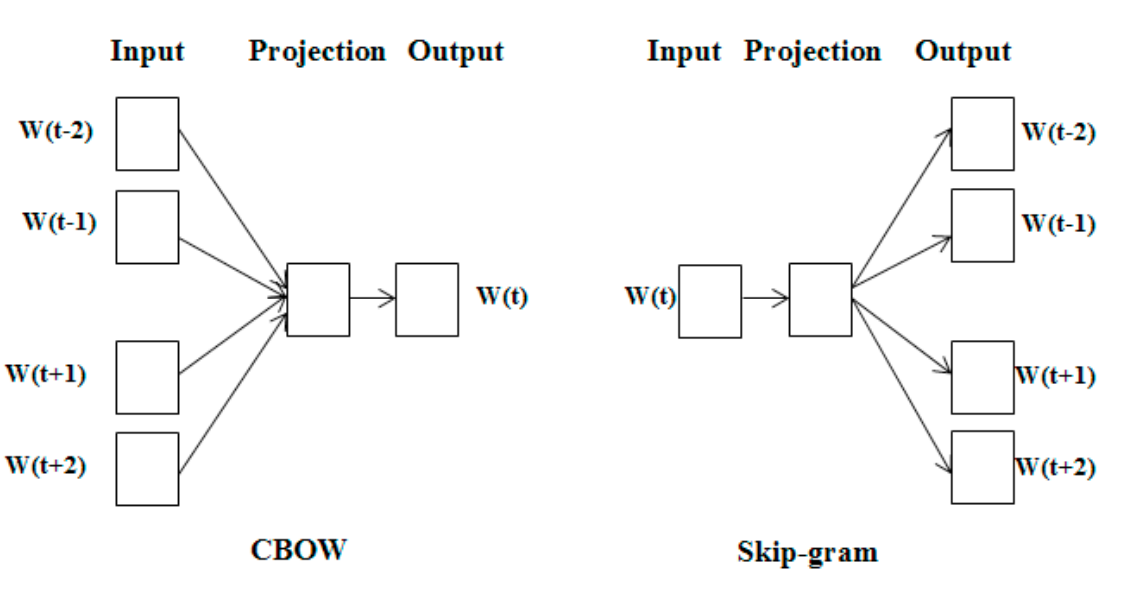
\includegraphics[width=0.5\linewidth]{texfiles//images/skip_gram_vs_cbow.png}
    \caption{CBOW vs Skip-gram word embedding models, \cite{jatnika2019word2vec}}
    \label{fig:enter-label}
\end{figure}

When using word embeddings in recurrent neural networks, it is usual to include what is called an embedding layer as the first layer of the network. The function of this layer is to train and tailor the word embeddings to better suit the specific task of the network. The reason I say tailor is because the amount of needed data and computational power to create and train word embedding set for a dictionary of any substantial size is quite large it is normal to use pre-trained word embedding datasets, and fine-tune these through the embedding layer to better suit the task of the specific network. As we were not sure as to what our task for the network would be specifically we decided a static pre-trained word embedding dataset would suffice, meaning we decided to omit the embedding layer and not train the embedding in the dataset any further to fine-tune them for our network. This will probably limit our results a bit, however, given we don't have any specific categories or themes in mind for our training data the, general word embeddings should suffice.
To take care of the translation to and from the vector space, and find the cosine similarity between word embeddings, we are using the \cite{Spacy} python library, which also provides us with a selection of pre-trained word embedding datasets. These datasets range from the smallest containing 50-dimensional word embeddings to the biggest containing 300-dimensional ones.
word embeddings

\section{Results}

\section*{Appendix - some math notes}

\subsection*{Backpropagation through time - BPTT}
Definitions:
\begin{align}
    \mathbf{a}^{(t)} &= \mathbf{b + Wh^{(t-1)} + Ux^{(t)}} \\
    \mathbf{h}^{(t)} &= activation(\mathbf{a}^{(t)})\\
    \mathbf{o}^{(t)} &= \mathbf{c + Vh}^{(t)} \\
    \mathbf{\hat{y}}^{(t)} &= softmax(\mathbf{o}^{(t)}) \\
    \mathbf{U} &= \text{input weights} \\
    \mathbf{W} &= \text{hidden weights} \\
    \mathbf{V} &= \text{output weights}
\end{align}


The goal is to maximize the probability of the observed data by estimating parameters (here: $\mathbf{U, V, W, b, c}$). The estimated parameters yielding the highest maximum likelihood are called the maximum likelihood estimates. These parameters can be estimated by minimizing the cross-entropy between the model distribution and the data. %To ease calculations, and because of the concavity of the problem, we derive the following cost-function:
This cross-entropy function, which is a function of inputs ($\mathbf{x}$) and outputs ($\mathbf{y}$), can be seen in (8).
\begin{align}
    &C\left(\{\mathbf{x}^{(1)},...,\mathbf{x}^{(\tau)}\}, \{\mathbf{y}^{(1)},...,\mathbf{y}^{(\tau)}\}\right) \\
    &= \sum_t C^{(t)} \\
    &= -\sum_t log\;p\left(y^{(t)}|\{\mathbf{x}^{(1)},...,\mathbf{x}^{(t)}\}\right) \\
\end{align}

Note: $\quad y^{(t)} \;\;$ is an entry in the output vector $\;\; \mathbf{\hat{y}}^{(t)}$ \par
The cost function is the negative log-likelihood function. Minimising this function is the same as maximum the likelihood of the parameters - not due to the log, but due to the negative prefix. The log in log-likelihood works, but I dont know why it is used? \par
Below we derive the gradients of the nodes in the computational graph from the deep learning book. These gradients must propagate backwards through time, from time $t=\tau$ down to $t=0$.
\par
The gradient of the cost function at the output, $\mathbf{o}$, at time \textit{t} is
\begin{align}
    \nabla_{\mathbf{o}^{(t)}} C &= \frac{\delta C}{\delta o^{(t)}}
    = \frac{\delta C}{\delta C^{(t)}}\frac{\delta C^{(t)}}{\delta o^{(t)}}
    = \hat{y}^{(t)} - \mathbf{1}_{i=y^{(t)}}
    % \text{i is indices in $\hat{y}^{(t)}$. The predicate at the end of the previous line makes sence if one considers for example the $\hat{y}^{(t)}$ consisting of probabilities for all the different characters.}
\end{align}

We have found a general expression for the gradien at the $\mathbf{o}^{(t)}$-nodes. The next step is to find an expression for the gradient of the final hidden (computational) node, at time $\tau$: $\mathbf{h}^{(\tau)}$. Its only descendant is $\mathbf{o}^{(\tau)}$, which means its gradient is solely dependent on this node, which makes it a good starting point for the later gradient calculations.

\begin{align}
    \nabla_{\mathbf{h}^{(\tau)}} C &= \left(\nabla_{\mathbf{o}^{(\tau)}}C\right) \frac{\delta \mathbf{o}^{(\tau)}}{\delta \mathbf{h}^{(\tau)}}\\
    &= \left(\nabla_{\mathbf{o}^{(\tau)}}C\right) \mathbf{V}\\
    \nabla_{\mathbf{h}^{(\tau)}} C &= \mathbf{V}^{\top} \left(\nabla_{\mathbf{o}^{(\tau)}}C\right)
    % \nabla_{\mathbf{h}{(\tau)}} C &= \mathbf{V}^{\top}\left(\hat{y}^{(\tau)} - \mathbf{1}_{i=y^{(\tau)}}\right) \\
\end{align}
Where all the right hand side terms are known from before. \par

The only nodes that need gradient computation now, are all the hidden states preceding the last. I.e., for $\mathbf{h}^{(t)}$, where $t = \{0,...,\tau-1\}$. For these time steps, the gradient is influenced by both the gradient at $\mathbf{o}^{(t)}$, as well as all the preceding hidden state gradients. Remember that the preceding hidden state of $\mathbf{h}^{(t)}$ is $\mathbf{h}^{(t+1)}$, which has preceding hidden state $\mathbf{h}^{(t+2)}$, and so on. We are calculating the gradient starting from $t=\tau-1$, working our way down to $t=0$: \par
% \begin{align}
%     \shortintertext{Denne linja kan være veldig feil}
%     \nabla_{\mathbf{h}^{(t-1)}} C &= \nabla_{\mathbf{h}^{(t)}} C + \nabla_{\mathbf{o}^{(t-1)}}C \\ 
%     \nabla_{\mathbf{h}^{(t-1)}} C &= \nabla_{\mathbf{h}^{(t)}} C \frac{\delta}{\delta} + V^{\top}\left(\nabla_{\mathbf{o}^{(t-1)}}C\right)
% \end{align}

\begin{align}
    \nabla_{\mathbf{h}^{(\tau-1)}} C &= \color{blue}\nabla_{\mathbf{o}^{(\tau-1)}}C \frac{\delta \mathbf{o}^{(\tau-1)}}{\delta \mathbf{h}^{(\tau-1)}} + \nabla_{\mathbf{h}^{(\tau)}}C \frac{\delta \mathbf{h}^{(\tau)}}{\delta \mathbf{h}^{(\tau-1)}} \\
    \nabla_{\mathbf{h}^{(\tau-2)}} C &= \color{red}\nabla_{\mathbf{o}^{(\tau-2)}}C \frac{\delta \mathbf{o}^{(\tau-2)}}{\delta \mathbf{h}^{(\tau-2)}} + \color{blue}\nabla_{\mathbf{h}^{(\tau-1)}}C \color{red} \frac{\delta \mathbf{h}^{(\tau-1)}}{\delta \mathbf{h}^{(\tau-2)}} \\
    \nabla_{\mathbf{h}^{(\tau-3)}} C &= \nabla_{\mathbf{o}^{(\tau-3)}}C \frac{\delta \mathbf{o}^{(\tau-3)}}{\delta \mathbf{h}^{(\tau-3)}} + \color{red}\nabla_{\mathbf{h}^{(\tau-2)}}C \color{black} \frac{\delta \mathbf{h}^{(\tau-2)}}{\delta \mathbf{h}^{(\tau-3)}} \\
    &= \nabla_{\mathbf{o}^{(\tau-3)}}C \frac{\delta \mathbf{o}^{(\tau-3)}}{\delta \mathbf{h}^{(\tau-3)}} + \color{red}\left(\nabla_{\mathbf{o}^{(\tau-2)}}C \frac{\delta \mathbf{o}^{(\tau-2)}}{\delta \mathbf{h}^{(\tau-2)}} + \color{blue}\nabla_{\mathbf{h}^{(\tau-1)}}C\color{red} \frac{\delta \mathbf{h}^{(\tau-1)}}{\delta \mathbf{h}^{(\tau-2)}} \right) \color{black} \frac{\delta \mathbf{h}^{(\tau-2)}}{\delta \mathbf{h}^{(\tau-3)}} \\
    &= \nabla_{\mathbf{o}^{(\tau-3)}}C \frac{\delta \mathbf{o}^{(\tau-3)}}{\delta \mathbf{h}^{(\tau-3)}} + \color{red}\left(\nabla_{\mathbf{o}^{(\tau-2)}}C \frac{\delta \mathbf{o}^{(\tau-2)}}{\delta \mathbf{h}^{(\tau-2)}} + \color{blue}\left(\color{blue}\nabla_{\mathbf{o}^{(\tau-1)}}C \frac{\delta \mathbf{o}^{(\tau-1)}}{\delta \mathbf{h}^{(\tau-1)}} + \nabla_{\mathbf{h}^{(\tau)}}C \frac{\delta \mathbf{h}^{(\tau)}}{\delta \mathbf{h}^{(\tau-1)}} \right)\color{red} \frac{\delta \mathbf{h}^{(\tau-1)}}{\delta \mathbf{h}^{(\tau-2)}} \right) \color{black} \frac{\delta \mathbf{h}^{(\tau-2)}}{\delta \mathbf{h}^{(\tau-3)}} \\
    \shortintertext{Generally:}
    \nabla_{\mathbf{h}^{(t)}} C &= \nabla_{\mathbf{o}^{(t)}}C \frac{\delta \mathbf{o}^{(t)}}{\delta \mathbf{h}^{(t)}} + \nabla_{\mathbf{h}^{(t+1)}}C \frac{\delta \mathbf{h}^{(t+1)}}{\delta \mathbf{h}^{(t)}}
    % &= \nabla_{\mathbf{o}^{(\tau-2)}}C \frac{\delta \mathbf{o}^{(\tau-2)}}{\delta \mathbf{h}^{(\tau-2)}} + \color{blue}\left(\nabla_{\mathbf{o}^{(\tau-1)}}C \frac{\delta \mathbf{o}^{(\tau-1)}}{\delta \mathbf{h}^{(\tau-1)}} + \nabla_{\mathbf{h}^{(\tau)}}C \frac{\delta \mathbf{h}^{(\tau)}}{\delta \mathbf{h}^{(\tau-1)}}\right)\color{black}\frac{\delta \mathbf{h}^{(\tau-1)}}{\delta \mathbf{h}^{(\tau-2)}}
    % \nabla_{\mathbf{h}^{(0)}} C &= \nabla_{\mathbf{o}^{(0)}}C + \nabla_{\mathbf{h}^{(\tau-3)}}C \\
\end{align}\par
Some parts of the equations above have been colored to emphasize the parts that we take with us from one gradient calculation to the next. \par
It is observable that the gradient at time $t$ is indeed dependent on all later time steps $t + 1, t + 2, t + n$, as well as the current output. The influence from current output can be seen before the first (+), while the influence from previous states can be observed after the first (+). \par

The final step is to calculate the gradient of the parameter nodes $\mathbf{U, W, b, V, c}$. To find these gradients, we must differentiate $\mathbf{h}^{(t)}$. Calculating the derivative of $\mathbf{h}^{(t)}$ involves differentiating the activation function using the chain rule. In the equations below, the chain rule is applied to differentiate the activations with respect to different parameters, but the activation function itself is not differentiated because it depends on which activation function in use. It is instead denoted as $\nabla_{activation}$.
\begin{align*}
    \nabla_\mathbf{c}C &= \sum_t \left(\nabla_{\mathbf{o}^{(t)}}C\right) \frac{\delta \mathbf{o}^{(t)}}{\delta \mathbf{c}^{(t)}} &&= \sum_t \left(\nabla_{\mathbf{o}^{(t)}}C\right) \cdot 1 \\
    \nabla_\mathbf{V}C &= \sum_t \left(\nabla_{\mathbf{o}^{(t)}}C\right) \frac{\delta \mathbf{o}^{(t)}}{\delta \mathbf{h}^{(t)}} &&= \sum_t \left(\nabla_{\mathbf{o}^{(t)}}C\right)\mathbf{h^{(t)}} \\
    \nabla_\mathbf{b}C &= \sum_t \left(\nabla_{\mathbf{h}^{(t)}}C\right) \frac{\delta \mathbf{h}^{(t)}}{\delta \mathbf{b}^{(t)}} &&= \sum_t \left(\nabla_{\mathbf{h}^{(t)}}C\right) \left(\nabla_{activation}\right) \cdot 1 \\
    \nabla_\mathbf{W}C &= \sum_t \left(\nabla_{\mathbf{h}^{(t)}}C\right) \frac{\delta \mathbf{h}^{(t)}}{\delta \mathbf{W}^{(t)}} &&= \sum_t \left(\nabla_{\mathbf{h}^{(t)}}C\right) \left(\nabla_{activation}\right) \cdot \mathbf{h}^{(t-1)} \\
    \nabla_\mathbf{U}C &= \sum_t \left(\nabla_{\mathbf{h}^{(t)}}C\right) \frac{\delta \mathbf{h}^{(t)}}{\delta \mathbf{U}^{(t)}} &&= \sum_t \left(\nabla_{\mathbf{h}^{(t)}}C\right) \left(\nabla_{activation}\right) \cdot \mathbf{x}^{(t-1)}\\
\end{align*}


The code written for BPTT is tricky to read. Below is conversions from math to code for gradient calculation of eq. (21):
\begin{align*}
    \nabla_{\mathbf{o}^{(t)}} C &= \hat{y}^{(t)} - \mathbf{1}_{i=y^{(t)}} &&\Rightarrow \texttt{w\_hy} \\
    \frac{\delta \mathbf{o}^{(t)}}{\delta \mathbf{h}^{(t)}} &= \mathbf{V} &&\Rightarrow \texttt{grad\_o\_Cost} \\
    \nabla_{\mathbf{h}^{(t+1)}} C &= \nabla_{\mathbf{o}^{(t+1)}}C \frac{\delta \mathbf{o}^{(t+1)}}{\delta \mathbf{h}^{(t+1)}} + \nabla_{\mathbf{h}^{(\tau)}}C \frac{\delta \mathbf{h}^{(t+2)}}{\delta \mathbf{h}^{(t+1)}} &&\Rightarrow \texttt{prev\_grad\_h\_Cost} \\
    \frac{\delta \mathbf{h}^{(t+1)}}{\delta \mathbf{h}^{(t)}} &= \mathbf{W} &&\Rightarrow \texttt{w\_hh} \\
    \nabla_{\mathbf{h}^{(t)}} C &&&\Rightarrow \texttt{grad\_h\_Cost} \\
\end{align*}

\begin{align*}
    z_t &= Ux_t + Wh_{t-1} + b_t \\
    h_t &=  \sigma(z_t) \\
    o_t &=  Vh_t + c_t \\
    y_t &=  \sigma(Vh_t + c_t) \\
    C^t &= C(y_t,\hat{y_t}) \\
    \frac{\delta C_t}{\delta W} &= \frac{\delta C_t}{\delta y_t}
    \cdot \sum^n_{k=1}\left[\frac{\delta h_t}{\delta h_.}\cdot\right] \frac{\delta h_k}{W}
\end{align*}


\bibliography{texfiles/refs}


\end{document}